\begin{par}

    \par \hspace{15pt} The VGG-based CNN classifier was able to provide some sensible results for the classification task after training of 50 epochs. The network was able to give around $76\%$ of accuracy upon the testing set and about $81\%$ on the training set on average of 3 to 4 training attempt. The model was trained on the LPD-5 cleansed dataset on an Nvidia GTX 1070 first, with parallel training with different hyperparameters on a different machine with an Nvidia Tesla T4. Training of 50 epochs usually takes about 7 hours on either GPU with no significant difference. However, the Tesla T4 was able to train the model with a larger batch size with the additional graphical memories, which usually leads to a slightly better training results. 
    
    \begin{figure}[H]
        \centering
        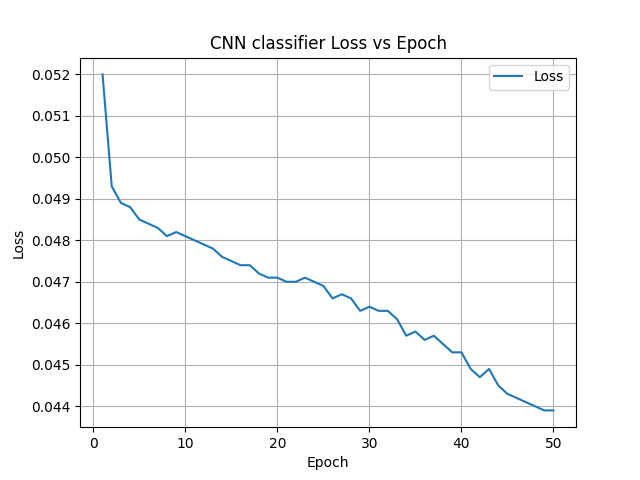
\includegraphics[width=4in]{image/loss_vs_epoch_train_log_2022-03-09_23-05-36}
        \caption{Loss Histogram of the CNN training}
        \label{fig:loss_hist}
    \end{figure}
    
    \par \hspace{15pt} Figure \ref{fig:loss_hist} shows the loss histogram of training the classifier model. According to the plot, the loss of the training is not plateaued at the ending training epoch, signifying that the model is still learning, yet at the end of 50 epochs, the model was able to give an output of around $80\%$ accuracy. Thus the group believe that with longer training time and better hardware accelerator, the model will be able to achieve better results. The group would try to investigate on further training with the next half of the project.

\end{par}